\documentclass[12pt]{article}
\usepackage[margin=1in]{geometry}
\usepackage{amsmath,amsthm,amssymb}
\usepackage{natbib}
\usepackage{graphicx}
\graphicspath{ {images/} }
 
\newcommand{\N}{\mathbb{N}}
\newcommand{\Z}{\mathbb{Z}}
\newcommand{\R}{\mathbb{R}}
\newcommand{\Indicator}{\mathds{1}}
\newcommand{\EX}{\mathbb{E}}
\newcommand{\Prob}{\mathbb{P}}

\author{Andrew Benton}
\title{Constant bounded approximation algorithms for stochastic inventory control}

\begin{document}

\maketitle

\section{Introduction}

\cite{levi:2007}, \cite{levi:2008} develop and advance the idea of \textit{Marginal Cost Accounting} and \textit{Cost Balancing}. Marginal Cost Accounting is a method where the total discounted cost of the current decision is computed and minimized. Although similar in effect as a \textit{Dynamic Programming} approach, it differs in that the future costs are separated into their components (holding, backorder, etc), and can be computed for one period without requiring the entire horizon to be solved. Cost Balancing allows for an efficient method of solving the resulting equations, and provides bounds of performance. \cite{hurley:2007} applies these models and shows that these bounds are strong.

\section{Stochastic Inventory Models}

\cite{levi:2007} present algorithms for the stochastic inventory control problem and the lot sizing problem. \cite{levi:2008} present algorithms for the capacitated stochastic inventory control problem. [TODO] multi-echelon inventory control problem. For all of these, they present an algorithm as well as worst case performance guarantees. 

\subsection{Stochastic Inventory Problem}

This problem has per unit holding costs $h_s$ and per unit lost sales costs $p_s$. Marginal cost accounting attributes some portion of the future costs directly to the decision made in the current period. Given the demand sequence $\{d_t\}_t$, a starting inventory $X_t$, the period $s$ holding costs $H^B_s(q_s)$ are computed from the current period to the end of the horizon. 
$$
	H_s^B(q_s) = \sum_{j=s}^T h_j \big[q_s - \big(\sum_{i=s}^j d_i - X_s\big)^+\big]^+
$$
The penalty costs $\Pi_s^B(q_s)$ are simplified by the observation that if too few items are bought during the current period, more can be purchased. Due to this, penalty costs only need to be computed for a single period.
$$
	\Pi_s^B(q_s) =  p_s [D_s - (X_s^B + q_s)]^+ 
$$
Using these equations, the Balancing Algorithm seeks the order size $q_s$ where these two costs are equal. That is:
$$
	l_s^B(q_s) = \pi_s^B(q_s)
$$
where $l_s^B(q_s) = \EX[H_s^B(q_s) \; | f_s]$ and $\pi_s^B(q_s) = \EX[\Pi_s^B(q_s) \; | f_s]$. \cite{levi:2007} show that when this $q_s$ is applied, the incurred costs are guaranteed to be twice of the optimal costs.  

\subsection{Lot Sizing Problem}

This problem has per unit holding costs $h_s$, per unit lost sales costs $p_s$, and a per order fixed cost $K$. The approach taken by Levi et al. (2007) seeks to separately balance the holding costs and ordering costs as well as the penalty costs and ordering costs. Here, the Balancing Algorithm provides two parameters: the inventory level at which to order, and the level to order up to (analagous to (s, S) in the exact formulation of this problem). An order is made if the backordering costs exceed $K$:
$$
	q_s^B = \min_{q} \{q \; : \; \pi_s^B(q_s) \leq K\} 
$$
The order size is then:
$$
	q_s^B = \max_{q_s} \{q \; : \; l_s^B(q_s) \leq K\} 
$$
\cite{levi:2007} show that when this policy is applied, the incurred costs are guaranteed to be three times of the optimal costs.  

\subsection{Capacitated Stochastic Inventory Problem}

This problem has per unit holding costs $h_s$, per unit lost sales costs $p_s$, and a maximum order size $Q_s$. This problem is effectively a generalization of the uncapacitated stochastic inventory problem, and the balancing algorithm treats it as such. 
[TODO: type up the equations]

\section{Analysis of Cost Functions}

\subsection{Marginal Holding Cost $l_s^B(q_s)$}

Computing $l_s^B(q_s)$ in the general case requires the computation of a $T - s$ dimensional integral. Traditional cubature algorithms have exponential complexity in dimensions, making such an integral unreasonable to compute. However, some conditions allow it to be reduced to $T-s$ integrals of fewer dimensions. Letting $\Phi$ be the (generally multivariate) distribution of forecast $f_s$: 
\begin{alignat*}{1}
	l_s^B(q_s) &= \EX [H_s^B(q_s) \; | \; f_s] \\
        &= \EX \bigg\{\sum_{j=s}^T h_j\bigg[q_s - \bigg(\sum_{i=s}^j D_i - X_s\bigg)^+\bigg]^+  \; | \; f_s \bigg\} \\
		&= \int_{u_s}^{\infty} \int_{u_{(s+1)}}^{\infty}\dots \int_{u_T}^{\infty}\sum_{j=s}^T h_j\bigg[q_s - \bigg(\sum_{i=s}^j u_i - X_s\bigg)^+\bigg]^+ d\Phi(u_s, u_{s+1}, \dots u_T)\\
	   &= \sum_{j=s}^T \int_{u_s}^{\infty} \int_{u_{(s+1)}}^{\infty}\dots \int_{u_j}^{\infty} h_j\bigg[q_s - \bigg(\sum_{i=s}^j u_i - X_s\bigg)^+\bigg]^+ d\Phi(u_s, u_{s+1}, \dots u_T)
\end{alignat*}
For independent demand, $l_s^B(q_s)$ and $\frac{d}{d q_s} l_s^B(q_s)$ can be expressed as $T - s$ integrals in one dimension:
\begin{equation}
	l_s^B(q_s) = \sum_{j=s}^T \int_{u_j=X_s}^{X_s + q_s} h_j\bigg(q_s + X_s - u \bigg) (d\Phi_s \star d\Phi_{s+1} \star \dots \star d\Phi_j)(u)
\end{equation}
\begin{equation}
	\frac{d}{d q_s} l_s^B(q_s) =  \sum_{j=s}^T h_j \int_{u =X_s}^{X_s + q_s}  (d\Phi_s \star d\Phi_{s+1} \star \dots \star d\Phi_j)(u)
\end{equation}
For distributions with closed-form convolutions (Normal, Exponential, etc), these equations can be evaluated efficiently. For dependent demand or distributions without closed-form convolutions, this integral cannot be computed efficiently and accurately without simulation or more advanced cubature algorithms. 

\subsection{Marginal/Forced Backordering Cost}

The difficulties seen here are similar to those faced in Section 3.1. 
\begin{alignat*}{1}
	\tilde{\pi}_s^B(q_s) &= \EX [\tilde{\Pi}_s^B(q_s) \; | \; f_s] \\
        &= \EX \bigg\{\sum_{j=s}^T p_j\bigg[\sum_{i=s}^j u_i - \bigg(X_s + q_s- X_s\bigg)^+\bigg]^+  \; | \; f_s \bigg\} \\
		&= \int_{u_s}^{\infty} \int_{u_{(s+1)}}^{\infty}\dots \int_{u_T}^{\infty}\sum_{j=s}^T h_j\bigg[q_s - \bigg(\sum_{i=s}^j u_i - X_s\bigg)^+\bigg]^+ d\Phi(u_s, u_{s+1}, \dots u_T)\\
	   &= \sum_{j=s}^T \int_{u_s}^{\infty} \int_{u_{(s+1)}}^{\infty}\dots \int_{u_j}^{\infty} h_j\bigg[q_s - \bigg(\sum_{i=s}^j u_i - X_s\bigg)^+\bigg]^+ d\Phi(u_s, u_{s+1}, \dots u_T)
\end{alignat*}

\subsection{Myopic Penalty Function $\pi_s^B(q_s)$}

$\pi_s^B(q_s)$ is a more manageable integral.
\begin{alignat}{1}
	\pi_s^B(q_s) &= \EX [\Pi_t^B(q_s) \; | \; f_s] \nonumber \\
		&= \EX \bigg\{ p_s [D_s - (X_s^B + q_s)]^+  \; | \; f_s \bigg\} \nonumber \\
		&= \int_{u_s=({X_s^B + q_s})}^{\infty} p_s (u_s - X_s^B - q_s) d\Phi_s(u_s) \\
	\frac{d}{d q_s} \pi_s^B(q_s) &=  - \int_{u_s=({X_s^B + q_s})}^{\infty} p_s d\Phi_s(u_s) \nonumber \\
		&= - p_s (1 - \Phi_s(X_s^B + q_s)) 
\end{alignat}

\subsubsection{Loss Function}

As an informal validation, the loss function was computed exactly, and using simulated results with 100 replicates. An arbitrary scenario was picked for this task. The results are plotted below:

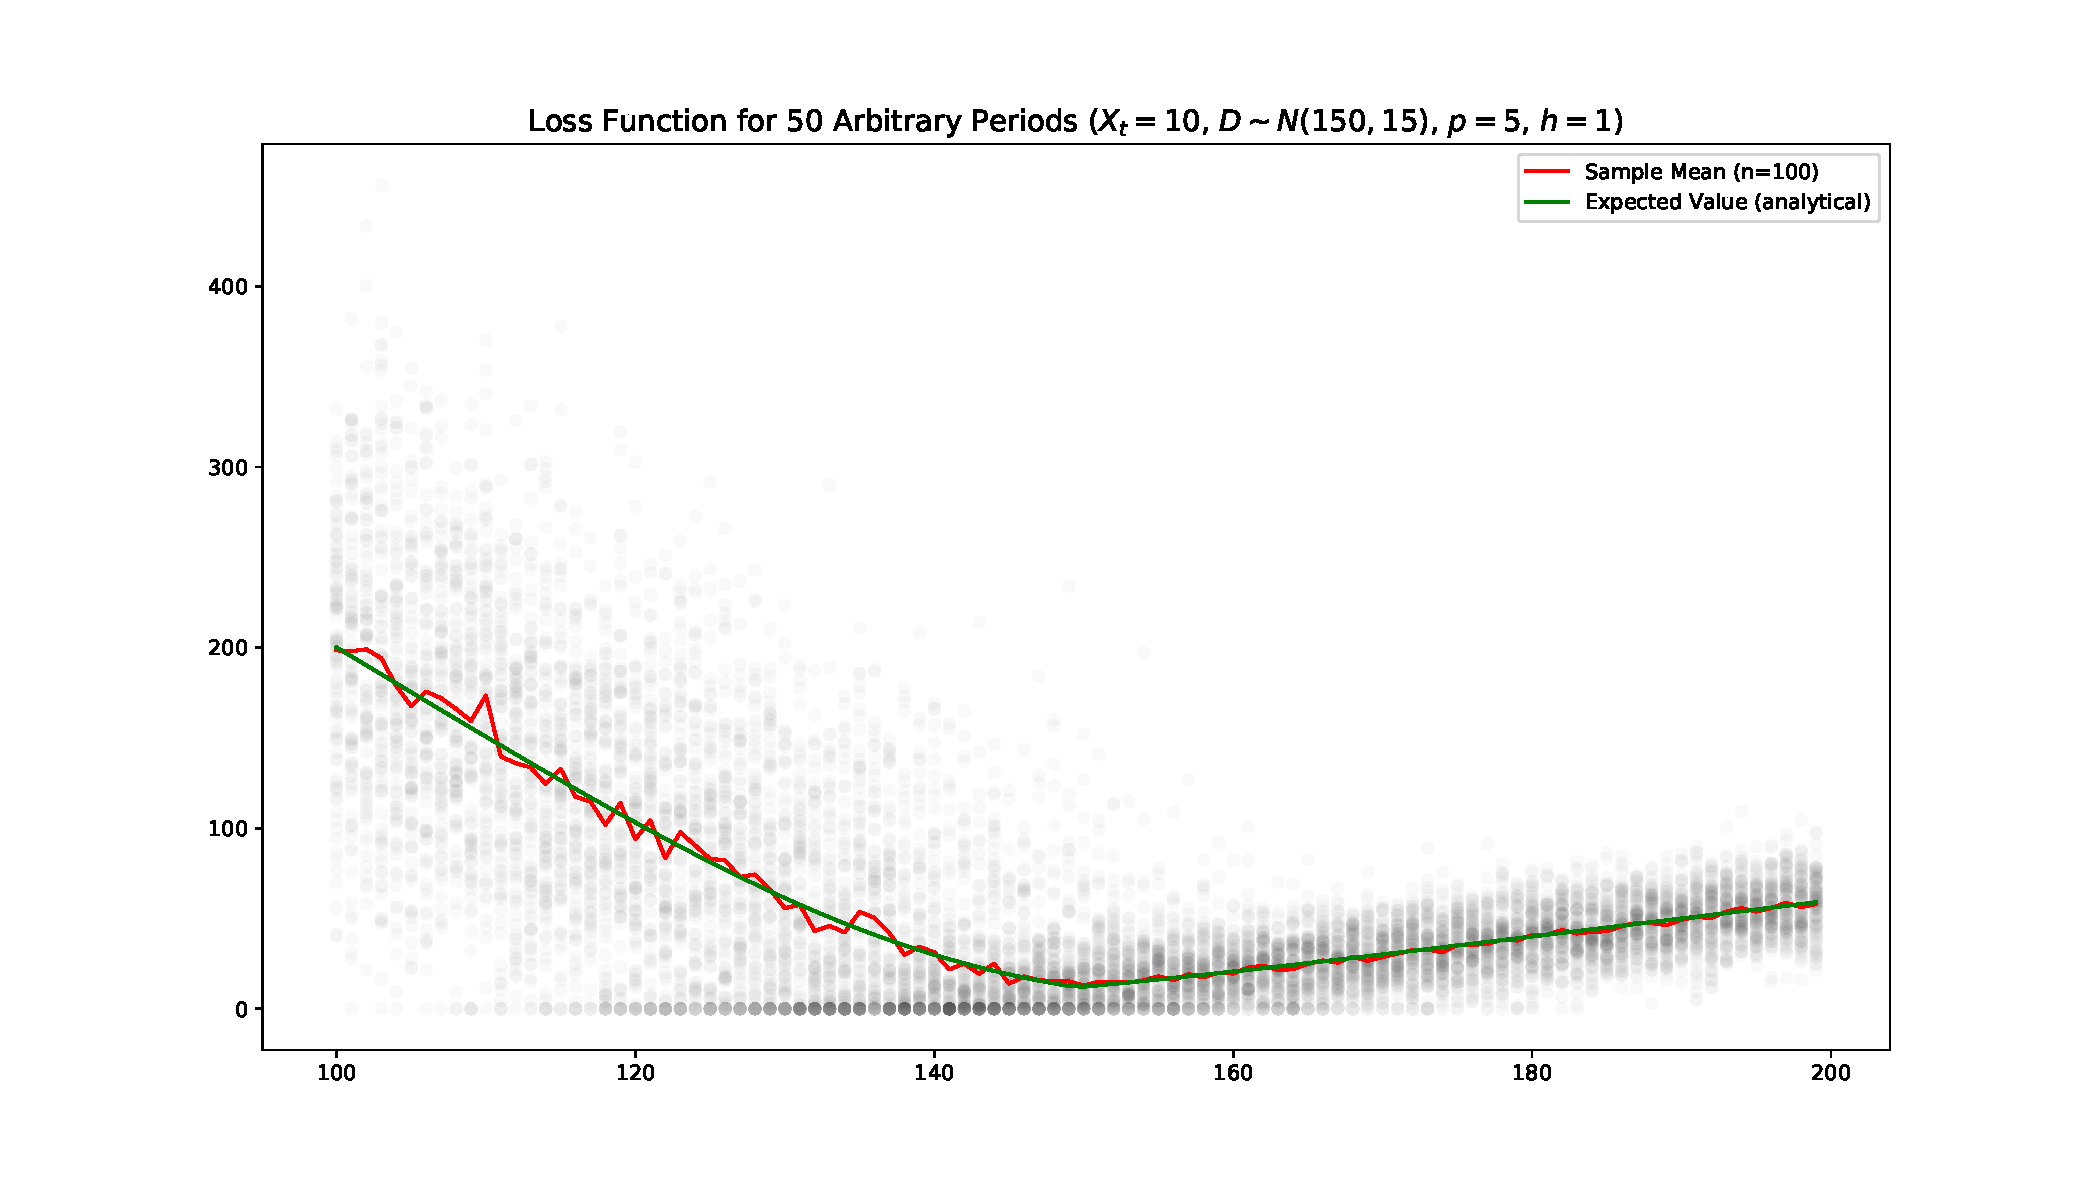
\includegraphics[width=\textwidth]{loss.pdf}

\section{Approximate Algorithms for Inventory Control}

When implementing these algorithms, I encountered many difficulties, particularly due to the intractability of one of the integrals resulting from the marginal cost accounting approach. Details on overcoming these difficulties are discussed in this section. 

\subsection{Dual Balancing Algorithm}

The Dual Balancing algorithm seeks the value $q_s^B$ such that: 
$$
	l_s^B(q_s^B) = \pi_s^B(q_s^B)
$$
Although there is an alternative convex minimization formulation, Levi et al suggests solving this in the root-finding formulation. The methods necessary to compute this root differ by the forecast type.

\subsubsection{Dual Balancing with Independent Forecasts}

Forecasting algorithms which provide independent forecast distributions allow for a more tractable solution. Practically speaking, this is a reasonable assumption: a large subset of forecasting algorithms (e.g. ARIMA variants) provide normally distributed forecasts. For this section we assume our forecasts are independently distributed. \\
\\
This would require locating the root of the following equation:
$$
	r_s^B(q_s^B) = l_s^B(q_s^B) - \pi_s^B(q_s^B) 
$$
Where the formulae for $l_s^B(q_s^B)$ and $\pi_s^B(q_s^B)$ can be found in equations (1) and (3). Levi et al suggests using the Bisection method (with linear convergence) to solve this. However, under our current assumptions, the derivative is available. This makes Newton-Raphson (with quadratic convergence) an option as well. The derivative for this equation is:
$$
	\frac{d}{dq_s^B} r_s^B(q_s^B) =  \frac{d}{d q_s} l_s^B(q_s) - \frac{d}{d q_s} \pi_s^B(q_s) 
$$
Where the formulae for $ \frac{d}{d q_s} l_s^B(q_s^B)$ and $ \frac{d}{d q_s} \pi_s^B(q_s^B)$ can be found in equations (2) and (4).\\
\\
Both Bisection and Newton-Raphson were tested for Scenario 1. The Bisection method required 49 evaluations of $r_s^B(q_s^B)$, while Newton-Raphson required 5 evalutions of both $r_s^B(q_s^B)$ and $\frac{d}{dq_s^B} r_s^B(q_s^B)$. The solved points $q_s^B$ differed by less than machine epsilon for both methods.

\subsubsection{Dual Balancing with General Forecasts}

For the general case, $l_s^B(q_s^B)$ cannot be computed without taking an integral over $T-s$ dimensions. This task cannot be done efficiently and accurately without some simulation approach (or more complicated procedures). \\
\\
To compute the root $q_s^B$, the Robbins-Monroe Algorithm was used. This requires the function $\hat{r}_s^B$, which evaluates $r_s^B$ for one demand sample, as well as an initial guess $q_s^0$. $q_s^B$ is then computed using the following equation:
$$
	q_s^i = q_s^{i-1} - \frac{1}{1 + i} \hat{r_s}^B(q_s^{i-1})
$$
This process can continue until convergence, or until some number of evalutations is reached. Because $q_s^i$ is not independent of $q_s^{i-1}$, it is generally useful to perform this process several times.\\
\\
Robbins-Monroe was used to recompute $q_s^B$ for the scenario discussed in the previous section. As shown in the plot below, convergence occurs within a few hundred iterations, and the final result is similar to the Newton-Raphson solution found previously. Because $\hat{r}_s^B$ is cheap to evaluate, the speed of this process is essentially limited by the random number generator. For this scenario, the Robbins-Monroe computing time was roughly an order of magnitude less than Newton-Raphson. 

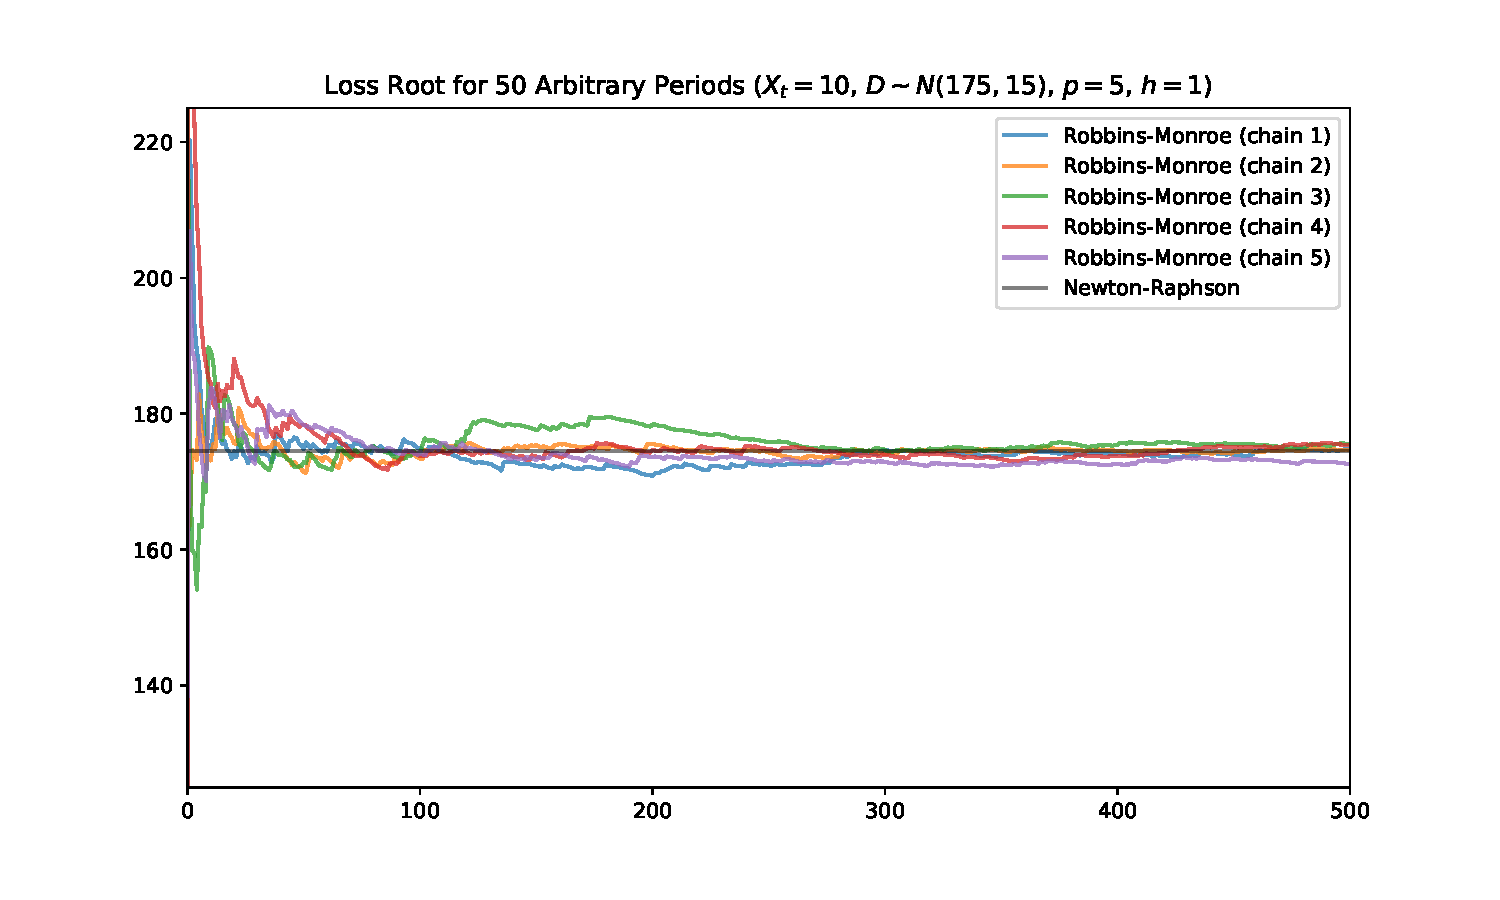
\includegraphics[width=\textwidth]{rbtraces}

\subsection{Triple Balancing Algorithm}

The Triple Balancing Algorithm seeks the value $q_s^B$ such that $q_s^B = \max\{q_s : l_s^B(q_s) \leq K\}$. This too is best viewed as a root-finding problem. As before, the computation needed to compute this will differ by the forecast type. 

\subsubsection{Triple Balancing Algorithm with Multivariate Normal Forecasts}

The approach taken here is similar to that of the Dual Balancing Algorithm. The root of the following equation must be located:
$$
	l_s^B(q_s) = K
$$ 
As above, there are some 

\bibliography{citations}
\bibliographystyle{plainnat}

\end{document}
